%! Author = Nectarios Chroniaris
%! Date = 2022-02-28

% Preamble
\documentclass[11pt]{article}
\usepackage[utf8]{inputenc}
\PassOptionsToPackage{hyphens}{url}\usepackage{hyperref}
\usepackage{listings}
\usepackage{verbatim}
\usepackage{makecell}
\usepackage{xcolor}
\usepackage{amsmath}
\usepackage{graphicx}

\newcommand{\ts}{\textsuperscript}

\definecolor{verylightgray}{gray}{0.95}

\definecolor{dkgreen}{rgb}{0,0.6,0}
\definecolor{gray}{rgb}{0.5,0.5,0.5}
\definecolor{mauve}{rgb}{0.58,0,0.82}

% https://tex.stackexchange.com/a/119864
\lstset{
    frame=single,
    framesep=6pt,
    framerule=0pt,
    xleftmargin=8pt,
    mathescape=false,
    backgroundcolor=\color{verylightgray},
    aboveskip=3mm,
    belowskip=3mm,
    showstringspaces=false,
    columns=flexible,
    basicstyle={\small\ttfamily},
    numbers=none,
    numberstyle=\tiny\color{gray},
    keywordstyle=\color{blue},
    commentstyle=\color{dkgreen},
    stringstyle=\color{mauve},
    breaklines=true,
    breakatwhitespace=true,
    tabsize=3
}

%! suppress = LineBreak
%! suppress = TooLargeSection
\begin{document}

    \title{magpieCTF 2022 - Turn-Key Writeup}
    \author{Nectarios Chroniaris}

    \maketitle


    \section{Preamble}\label{sec:preamble}

    The intended solve, as documented on \href{https://github.com/infosec-ucalgary/magpieCTF2022-public/tree/main/challenges/networks/turn-key}{magpieCTF's public GitHub repo}, involves renting/using servers that are physically close to the vaults, in order to get each request to complete in the required 300 or so milliseconds.

    \bigskip

    However, by taking some clever shortcuts in the design of the protocol, we can reduce round-trip delays and otherwise unnecessary overhead, to squeeze the total delay under the required amount (yes, even for the server in Bangalore!).


    \section{Abridged Solution}\label{sec:abridged-solution}

    \begin{enumerate}
        \item Read the specification and understand what messages are required to fulfill the protocol.
        \begin{itemize}
            \item Use \verb`nmap` to scan the vault servers to see which port the protocol is hosted under.
            \item \verb`nmap -p 1-65535 -T4 -A -v vault1.momandpopsflags.ca`
            \item i.e.\ ``scan all ports from 1--65535, be aggressive (\verb`-T4`, \verb`-A`) and log verbosely''.
        \end{itemize}
        \item After finding the correct port (thankfully they are all the same!), try to connect with \verb`nc` to see if it works.
        \begin{itemize}
            \item \verb`nc vault1.momandpopsflags.ca 5555`
            \item Test out the protocol, realize that your human fingers are much too slow to get the partial flag.
        \end{itemize}
        \item Start to write a script in your programming language of choice that can do TCP socket programming.
        \begin{itemize}
            \item The easiest IMO is Python 3, using the \verb`socket` library.
            \item Don't worry about efficiency in this step, just make sure that it works (the protocol successfully terminates).
            \item If you can get one vault, great! Remember we have to get all 3 at the same time.
        \end{itemize}
        \item Find room to improve efficiency and reduce overhead.
        \begin{itemize}
            \item Realize that you don't have to waste time reading, writing, and reading, and writing before something useful happens. You can just \textbf{immediately} send BOTH messages since the first two responses from the server are neither useful nor have any dynamic information.
            \item Remember it's fine to hardcode stuff here, because we want to break this specific protocol, and not have a general solution!
        \end{itemize}
        \item Run against all the servers at the same time to get all the necessary information for the key.
        \begin{itemize}
            \item Assuming your script is fast enough, you can run it all from the same machine using shell trickery:
            \item \verb`python3 <script> vault1 &` \\
            \verb`    python3 <script> vault2 &` \\
            \verb`    python3 <script> vault3 & wait`
        \end{itemize}
        \item Decrypt the flag using the 3-part key, initial value, and ciphertext from the vaults, using any tool of your choice.
        \begin{itemize}
            \item \href{https://gchq.github.io/CyberChef}{CyberChef is pretty convenient}, but any tool works, as there is nothing special going on here besides the key being split up into 3 pieces.
        \end{itemize}
    \end{enumerate}

    \pagebreak


    \section{Full Solution \& Thought Process}\label{sec:full-solution-thought-process}

    \subsection{Specification}\label{subsec:specification}

    Every good protocol starts off with a specification. We want to read this thoroughly and make sure we understand it, because then scripting will be easier. Here we note that:

    \begin{itemize}
        \item There are 3 vaults at different addresses.
        \item The protocol does not seem to rely on any other application-level protocol (like HTTP, for example), so it's likely just raw TCP messaging.
        \item The protocol involves us sending strings back to one another.
        \item In the final step we have to send a challenge string back.
        \begin{itemize}
            \item This means we have to make sure we read the data the server sent us so we can send it back.
        \end{itemize}
        \item There is no mention of what port(s) this service runs on, so we will have to find this ourselves.
        \item We have to get responses from all servers within 2.4s or else the encryption rotates.
        \item We know what output to expect in both the successful and unsuccessful cases.
    \end{itemize}

    \subsection{Finding Ports}\label{subsec:finding-ports}

    Fresh off our exciting specification adventure, it seems that the first step is to find where the service we want is hosted. We know the IP addresses (\verb`vaultX.momandpopsflags.ca`), but not the port.

    Pick one of the three servers to scan, and use any port scanning tool of your choice. I chose to use \verb`nmap`, since it was installed on my system.

    \begin{lstlisting}[gobble=8,label={lst:nmap-command}]
        $ nmap -p 1-65535 -T4 -A -v vault1.momandpopsflags.ca
    \end{lstlisting}

    \pagebreak

    \noindent A quick explanation of the options:

    \begin{table*}[h!]
        \centering
        \label{tab:nmap-command}
        \begin{tabular}{|r|l|}
            \hline
            \textbf{Flag} & \textbf{Description}                            \\ \hline
            \verb`-p N-M` & scan ports from \verb`N` to \verb`M`            \\ \hline
            \verb`-T4`    & Aggressive timing template, speeds up execution \\ \hline
            \verb`-A`     & Aggressive scan, gives more information         \\ \hline
            \verb`-v`     & Verbose logging                                 \\ \hline
        \end{tabular}
    \end{table*}

    After running this (it might take a couple of minutes!) you should see an open TCP port at 5555. That looks pretty out-of-place, so that's probably the one we want. In the next section we'll verify this by using netcat (\verb`nc`) to poke the service and see if it's the right one.

    \subsection{Playing Around With netcat}\label{subsec:playing-around-with-netcat}

    Now that we've scanned all the ports, we want to test to see if we have the right one, and that we're talking to the right protocol. The likeliest port from the scan was 5555, so we try to connect using a tool like \verb`netcat`.

    \verb`netcat` is a very useful tool for testing arbitrary TCP/UDP connections. In the \hyperref[subsec:specification]{specification section}, we didn't find any evidence of an application-layer protocol and figured it was implemented using raw TCP messages. \verb`netcat` is perfect for this use-case.

    \bigskip

    Using the following command we can establish a connection and start sending messages:

    \begin{lstlisting}[gobble=8,label={lst:netcat-command}]
        $ nc vault1.momandpopsflags.ca 5555
    \end{lstlisting}

    After running this, you should immediately see a message from the server, ``\verb`oh hai!`''. This matches exactly with what we were expecting from the specification, so we know we're in the right place. The terminal appears to block, but that's because it's waiting for us to type something to send to the server.

    At this point it's a good idea to emulate the protocol to gain understanding about what exactly the server expects in terms of messages, etc. With TCP messages like this, you'll want to make sure you end your message with a newline so that it is sent. This particular point will be important later, but for the purposes of \verb`netcat`, it is sufficient just to hit return/enter.

    You may try to interact with all 3 vaults, but a cursory probe (just connecting, not going through the whole protocol) reveals that the services seem to be exactly the same, and are hosted on the same port on all 3 vaults (5555).

    \bigskip

    After manually playing around with the protocol (and likely getting the ``unsuccessful'' output at the end), it's now time to script, so we can get the outputs in the required amount of time.

    \subsection{Naive Script}\label{subsec:naive-script}

    In this section \textbf{all you want to focus on is correctness}. There's no point in optimizing a broken program, so take it one step at a time. Here I am going to use Python 3 and the \verb`socket` library, mostly because I am familiar with it, and python scripts have a fast turnaround time (no need to set up build tools, etc.)

    First, we start off by establishing a connection to the vault, assuming that \verb`host` and \verb`port` are defined (these can be CLI arguments):

    \begin{lstlisting}[gobble=8,label={lst:script-establish},language=Python]
        import socket

        with socket.socket(socket.AF_INET, socket.SOCK_STREAM) as s:
            ip = socket.gethostbyname(host)
            s.connect((ip, port))
    \end{lstlisting}

    After this the server should already be sending us messages, and we should be set up to read them. Following the specification exactly, we read the ``\verb`oh hai!`'' message:

    \begin{lstlisting}[gobble=8,label={lst:script-reading-first},language=Python]
        server_data = s.recv(4096)    # 4096 is the buffer size
        print(server_data)            # b'oh hai!\n'
    \end{lstlisting}

    After reading \footnote{For the sake of simplicity, I am omitting the necessary idiom for \texttt{s.recv()}. The call usually blocks while the socket is open, requiring the use of a while loop and null checking. The full code can be viewed \hyperref[sec:full-optimized-code]{at the end of the document} or attached as a file alongside this report.} and printing the output (optional!) we can see that we get a bytestring representation of the message from the socket. We continue implementing the protocol, sending our strings next:

    \begin{lstlisting}[gobble=8,label={lst:script-writing-first},language=Python]
        s.sendall(b"INITIALIZE CONNECTION\n")
    \end{lstlisting}

    Here's where that newline comes into play. Since we're trying to script this, we \textbf{must} include a trailing newline in our message or else the TCP socket on our end will hang waiting for the rest of our message. This was the source of some confusion when creating my script, so watch out for that if you find that your program hangs prematurely.

    \bigskip

    By alternating between \verb`s.sendall()`'s and \verb`s.recv()`'s, you can pretty easily implement the protocol correctly. Note that when the server sends you the challenge string you have to extract it and send it back. You can either use regex capture groups or hardcode the indices to slice the challenge string out of the server response. The following is an example in regex:

    \begin{lstlisting}[gobble=8,label={lst:regex-extract},language=Python]
        server_data = s.recv(4096)
        match = re.findall(b'challenge string (.{7}\\n)', server_data)
        if match:
            return match[0]
    \end{lstlisting}

    Hopefully by now you should have a script that works (in terms of receiving a successful output), at least for one of the 3 vaults. That's perfectly normal since part of the challenge here is that the vaults are spread across the world. The important part here is making sure your script is correct.

    \subsection{Improved Script}\label{subsec:improved-script}

    This section describes what I think to be the crux of this unique solution to this challenge. As mentioned before, the intended solve is to rent/use a VPS that is physically close to the vaults. In fact, during the CTF, I really tried to consider this solution. At the time, my script worked for all vaults except the one in Bangalore, so I spent about 30 minutes on Google, trying to research my options on VPS hosting in India. I figured that there might have been a company that at least offered free trials, but was ultimately not able to find a service that had an easy way to rent or try out a VPS just for a couple of minutes.

    \bigskip

    In an effort solely motivated by my desire to not spend any money \ts{how can you blame me? :-P}, I decided to look at the script I wrote and see if there was \textbf{any} places where I could improve the efficiency or reduce overhead. I figured I was fighting a losing battle, because Python and efficiency don't always go hand-in-hand. I was even prepared to rewrite my protocol in C, in the case that nothing I did worked. Nevertheless, I pressed on.

    \bigskip

    In general, I had two ``epiphanies'' when it came to the protocol that I wrote, that ultimately led me to the solution you're reading.

    The first has to do with the leading end of the protocol. Recall that you have to do this ``handshake'' of sorts with the server until you get to the part where it sends you the flag. This process involves you reading an ``\verb`oh hai!`'', sending a ``\verb`INITIALIZE CONNECTION`'', reading a ``\verb`Connection successfully...`'', and finally ending with you sending a ``\verb`SEND FLAG`''. Notice that no matter when you establish this connection, these messages are \textbf{exactly the same, every single time}. So why are we wasting time doing this TCP dance (read, write, read, write) when (a) we deterministically know what commands we have to send, and (b) we don't really care for the first two server messages to begin with?

    This leads to the first improvement -- IMMEDIATELY sending the commands we need to send to fulfil the protocol, right out of the gate:

    \begin{lstlisting}[gobble=8,label={lst:first-efficiency},language=Python]
        s.connect((ip, port))

        # Send both commands IMMEDIATELY, not caring whether there is data to read or not
        s.sendall(b"INITIALIZE CONNECTION\n")
        s.sendall(b"SEND FLAG\n")

        # get_challenge() reads the socket for data, and extracts the challenge string.
        # we just send the challenge string right back (part of protocol)
        s.sendall(get_challenge(buffer_size, s))
    \end{lstlisting}

    This seems dirty, as if we're betraying some strange TCP god out there, for daring to break from the usual structure. But if you think about it, TCP doesn't actually care if we read data from the socket or not. On one hand, the server is oblivious to our shenanigans, because from its perspective, it's already sent the data to us, and it has no idea if we chose to read it or not. The data it sent to us is just sitting in out TCP buffer, waiting patiently. On the other hand, we've already sent our data (likely before any data \textbf{actually} arrives in our TCP buffer), and the server has no idea if we sent this data in response to reading their messages or not.

    In other words, what we're doing here is making sure we're not \textbf{wasting} time \textit{blocking} the execution of our program while waiting for data from the server we're ultimately going to throw away. We're sending it anyway, pretending as if we read what the server wrote and responding accordingly.

    \pagebreak

    The following is a form of a sequence diagram that illustrates how exactly we benefit from such an optimization. The vertical axis represents time, but it is very \textbf{not} to scale:

    \noindent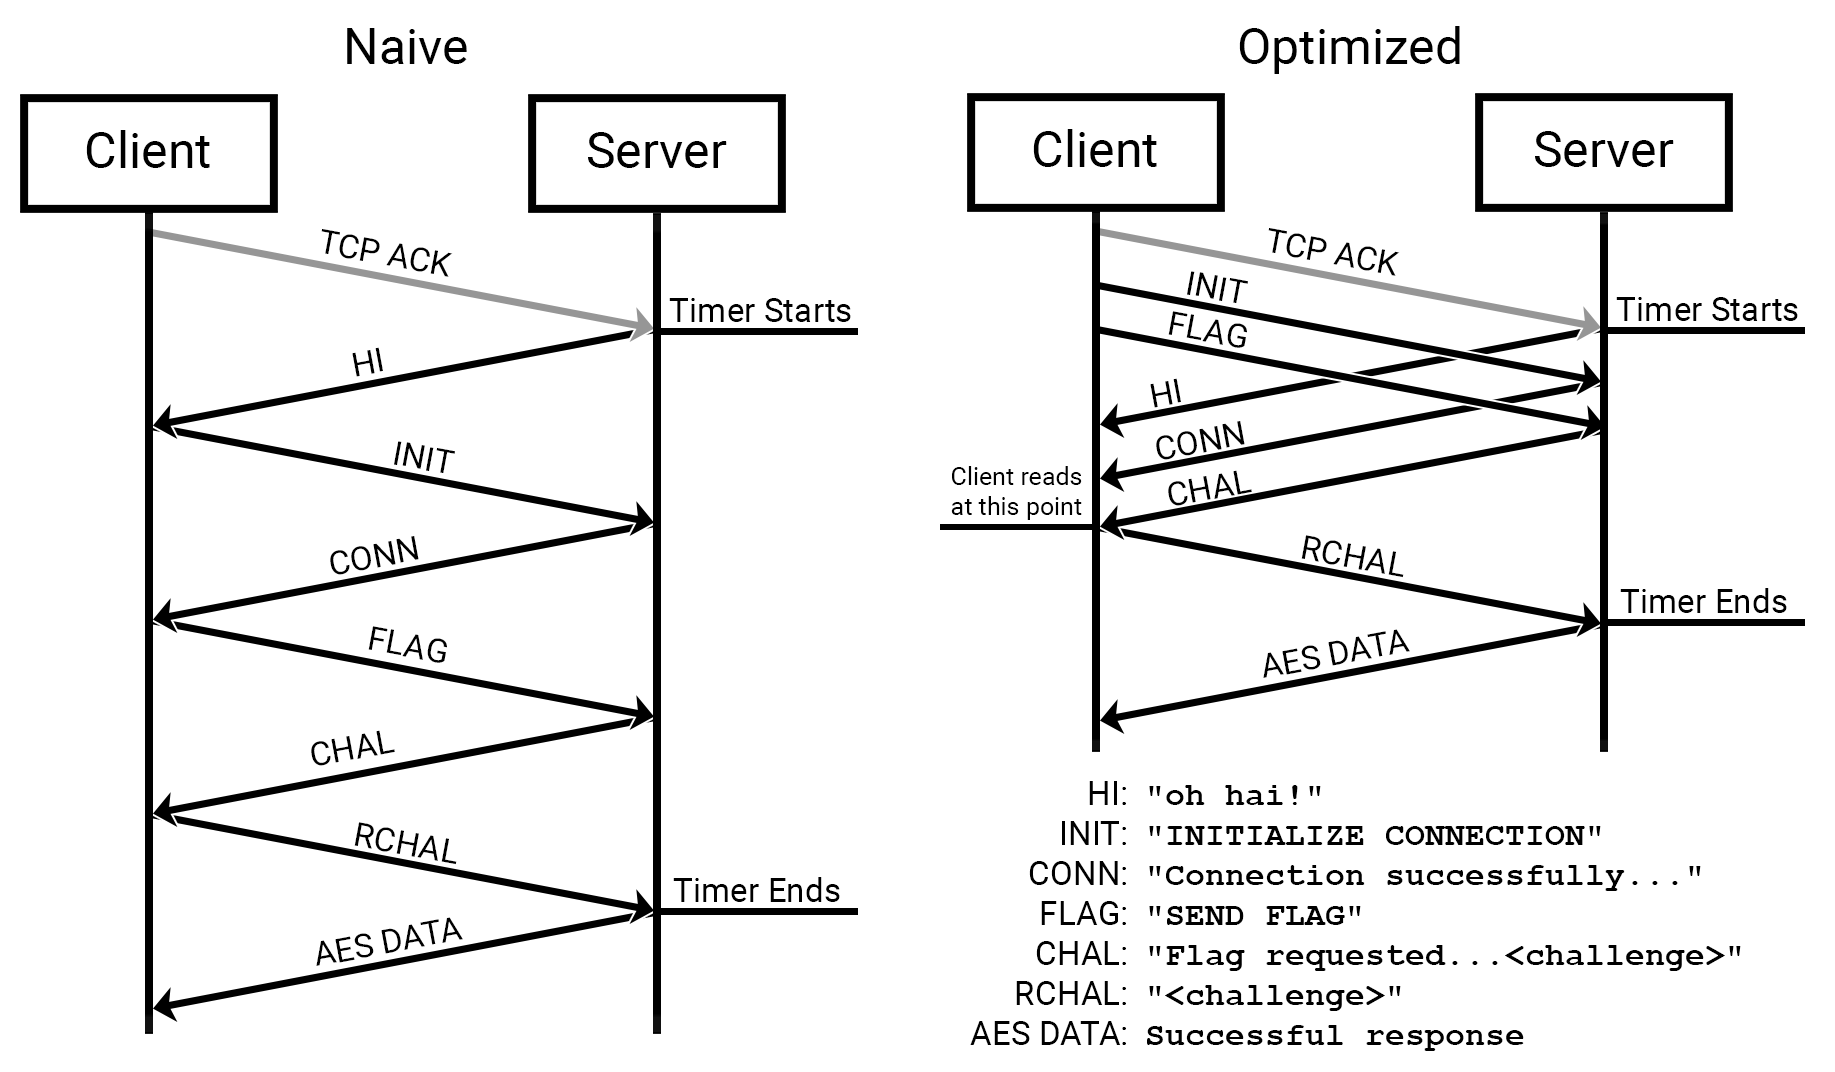
\includegraphics[width=\textwidth]{images/network_diagram}

    \noindent Note that in the optimized protocol:
    \begin{itemize}
        \item TCP ACK, INIT, and FLAG are sent pretty much at the exact same time
        \item The client only starts reading after a total of 3 messages are sent from the server
    \end{itemize}

    However, even after this I was still not able to get the vault in Bangalore. I was about 50--100ms outside the window, so I clearly had to find more room to improve. I have to give credit to one of my CTF teammates, Mark Holmstrom, who nudged me in the right direction with this particular optimization. We were talking over voice chat, and as I was \href{https://en.wikipedia.org/wiki/Rubber_duck_debugging}{explaining my progress so far}, he helped me realize that I was wasting time blocking when I was sending my initial messages. In particular, we're concerned with the following two lines:

    \begin{lstlisting}[gobble=8,label={lst:second-efficiency-1},language=Python]
        s.sendall(b"INITIALIZE CONNECTION\n")
        s.sendall(b"SEND FLAG\n")
    \end{lstlisting}

    Notice how I duplicated the \verb`sendall()` method. This seems pretty innocent at first glance, until you realize that the \href{https://docs.python.org/3/library/socket.html#socket.socket.sendall}{method is blocking}. That makes sense, because you want to make sure as a TCP participant you are making a best-effort to send all the bytes you want to send. However, that's bad for us, because we've duplicated the call --- meaning we're wasting time blocking on the second call when the information from the second call could have been included in the first:

    \begin{lstlisting}[gobble=8,label={lst:second-efficiency-2},language=Python]
        s.sendall(b"INITIALIZE CONNECTION\nSEND FLAG\n")
    \end{lstlisting}

    This frees us up from blocking a second time, not to mention we've probably removed some extra overhead that the \verb`.sendall()` method adds. The important thing to realize here is that TCP messages are effectively just bytestreams delimited by newlines, so it makes no semantic difference to bundle them together like this --- the server will read it in the same way.

    \bigskip

    As a bonus, a minor change I also made was replacing \hyperref[lst:regex-extract]{the regex method of extracting the challenge string} with a hardcoded string slicing solution:

    \begin{lstlisting}[gobble=8,label={lst:regex-efficiency},language=Python]
        if server_data[-15:-12] == b'str':
            return server_data[-8:]
    \end{lstlisting}

    Note that I made this change in conjunction with the \verb`sendall()` change, so I am unsure if this actually impacted the results. Side note: If you're screaming at me right now about hardcoding these indices, good --- that means your programmer senses are working correctly. In this case though it's justified because our aim is to break \textbf{this particular} protocol, and not have a general solution.

    \subsection{Turn All The Keys!}\label{subsec:turn-all-the-keys}

    Assuming you did everything right, you can successfully complete the protocol on all three servers. Great! All we need to do now is to execute 3 instances of our script, each pointed at a different vault, so we can get the AES information at the same time.

    We can use some shell trickery to achieve this, assuming you have the address of the server passed in as an argument:

    \begin{lstlisting}[gobble=8,label={lst:parallel-commands},language=Bash]
        $ python3 turn-key.py vault1.momandpopsflags.ca &
            python3 turn-key.py vault2.momandpopsflags.ca &
            python3 turn-key.py vault3.momandpopsflags.ca & wait
    \end{lstlisting}

    The \verb`&` character (very distinct from \verb`&&`) in most shells means ``execute in the background as a job'', preventing the shell from blocking until the first command executes. This allows us to ``schedule'' 3 commands so they execute roughly at the same time. The \verb`wait` command at the end there just tells the shell to wait for all its children to finish before it unblocks. This just makes the terminal output a bit cleaner, but it's not at all required.

    Assuming all 3 instances of the program succeeded, you should get an output similar to the following (sans any debug text or extraneous characters):

    \begin{lstlisting}[gobble=8,label={lst:server-output}]
        (1/3): 0x9DEFE0C566FE0264664BE
        IV: 0x4F5C25C4954F273472EC67AC494DADBD
        Ciphertext: 0x917774AA5412A434FA9EC619585D07E8DF1A48952E15ACCFD70
                        2F7B47F2C8610685164ACF4C4CE919C4F436615CFD275

        (2/3): 0x44D8BFCD0F625A8182A13
        IV: 0x4F5C25C4954F273472EC67AC494DADBD
        Ciphertext: 0x917774AA5412A434FA9EC619585D07E8DF1A48952E15ACCFD70
                        2F7B47F2C8610685164ACF4C4CE919C4F436615CFD275

        (3/3): 0xFEE73E2A20D92242FA45B5
        IV: 0x4F5C25C4954F273472EC67AC494DADBD
        Ciphertext: 0x917774AA5412A434FA9EC619585D07E8DF1A48952E15ACCFD70
                        2F7B47F2C8610685164ACF4C4CE919C4F436615CFD275
    \end{lstlisting}

    We can verify that we've gotten data from \textbf{the same rotation} by checking if all the \verb`Ciphertext` and \verb`IV` values match -- which in this case, they do. Victory! Now all we have to do is to decipher the 3-part AES ciphertext using all of this information.

    \subsection{Decrypting the Flag}\label{subsec:decrypting-the-flag}

    Now that we have all the information from the servers, it's time to stitch the key together, and try to decrypt the ciphertext with it and the initial value (IV). The key goes together following the prompts we have from the servers (1/3, then 2/3, then 3/3). Note that I've broken the lines up, so it fits on the page:

    \begin{lstlisting}[gobble=8,label={lst:aes-key}]
        Key: 0x9DEFE0C566FE0264664BE44D8BFCD0F6
                25A8182A13FEE73E2A20D92242FA45B5
    \end{lstlisting}

    \pagebreak

    Once we have the key, we can use something like \href{https://gchq.github.io/CyberChef}{CyberChef} to perform the decryption. But if you're feeling adventurous you can use \verb`openssl`, \verb`gpg`, or any tool of your choice. Here's a sample output of the decryption process with CyberChef:

    \noindent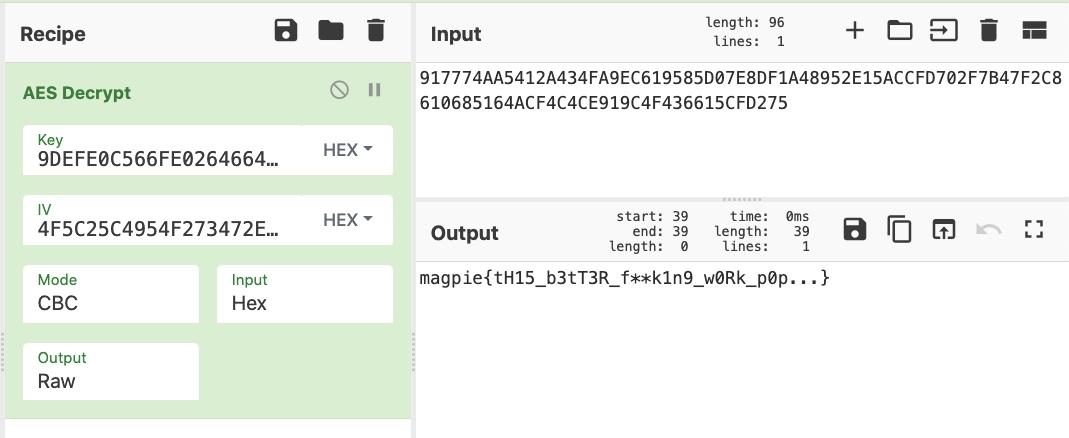
\includegraphics[width=\textwidth]{images/cyberchef}

    Perfect, we got the flag, all without renting a single server! My wallet survives another day longer.

    \section{Conclusion}\label{sec:conclusion}

    Thanks to James Lowther and Jeremy Stuart for making such a fun challenge. I had a lot of fun solving it, and a lot of fun doing this writeup! Hopefully it's not too long of a report :-P\@.

    \pagebreak

    \appendix


    \section{Full Optimized Code}\label{sec:full-optimized-code}

    \begin{lstlisting}[gobble=8,label={lst:full-code},language=Python,basicstyle={\scriptsize\ttfamily}]
        import socket
        import sys

        def main(argv):
            # Argument checking
            if len(argv) < 1:
                print("You must provide the host as an argument!", file = sys.stderr)
                return

            # Host grabbed from CLI argument, port is the same for all 3 vaults
            host = argv[0]
            port = 5555
            buffer_size = 4096

            # Open a TCP socket and resolve the IPof the host we got from the CLI
            with socket.socket(socket.AF_INET, socket.SOCK_STREAM) as s:
                ip = socket.gethostbyname(host)

                # Establish the connection (3-way handshake)
                s.connect((ip, port))

                # First attempt (introduces extra overhead)
                # s.sendall(b"INITIALIZE CONNECTION\n")
                # s.sendall(b"SEND FLAG\n")

                # Send both commands IMMEDIATELY, not caring whether there is data to read or not
                # bundle them both together to avoid extra overhead from sendall() being called twice
                s.sendall(b"INITIALIZE CONNECTION\nSEND FLAG\n")

                # get_challenge extracts the challenge string from the data the server sent us, and we just send it right back (part of protocol)
                s.sendall(get_challenge(buffer_size, s))

                # Read the response from the server after replying with the challenge string (hopefully we were quick enough!)
                res = get_response(buffer_size, s)
                print(res)

        def get_challenge(buffer_size, s) -> bytes:
            """Continues to read data from the socket, until we recognize the challenge string."""
            server_data = b''

            while True:
                # recv() blocks if there is no more data left to read, and the socket is still open
                server_data += s.recv(buffer_size)

                # First attempt (re library **might** not be as performant as string slicing)
                # match = re.findall(b'challenge string (.{7}\\n)', server_data)
                # if match:
                #     return match[0]

                # This is very hardcoded, but that's fine because we're just trying to break THIS protocol.
                # Sample bytestring: b'...with challenge string Z6D0N38\n' (remember, the `\n` is one character!)
                # They all have the same structure so if we check a slice of the output and get "str", we know that:
                # - We've read everything that the server has to send
                # - Our next command will be aligned properly
                if server_data[-15:-12] == b'str':
                    # Remember requests NEED to have a \n at the end to be considered "submitted", so we include that.
                    # i.e. 7 chars for the challenge, + 1 for the \n.
                    return server_data[-8:]

        def get_response(buffer_size, s):
            """Gets the final response from the server, assuming the rest of the protocol executed correctly."""
            server_data = b''

            try:
                while True:
                    # Keep reading data until a \n. Honestly this is a pretty flaky solution because there are 7 \n's in a successful final string, but the chances of a buffered read with a 4096 byte buffer ending on one of those intermediate ones is quite low, at least experimentally.
                    # If you run into problems, either remove it and ^C it yourself, OR use something like socket.select(). This worked for me, though.
                    server_data += s.recv(buffer_size)
                    if not server_data or server_data[-1] == ord(b'\n'):
                        break

                return server_data

            # In case something happens that causes us to block waiting for more data (can sometimes happen), a ^C will print what we captured already
            except KeyboardInterrupt:
                return server_data

        if __name__ == '__main__':
            # Removes program name from sysargs
            main(sys.argv[1:])
    \end{lstlisting}

\end{document}
